\documentclass[a4paper]{article}

\usepackage[utf8]{inputenc}
\usepackage[T1]{fontenc}
\usepackage[italian]{babel}

\usepackage[margin=4.2cm, top=1.5cm, bottom=2.5cm]{geometry}

\usepackage{siunitx}
\usepackage{amsmath}
\usepackage{amssymb}
\usepackage{xfrac}
\usepackage{esint}
\usepackage[hidelinks]{hyperref}
\usepackage{graphicx}
\usepackage[font={sf}]{caption}
\usepackage{pdflscape}
\usepackage{makecell}
\usepackage{float}
\usepackage{subfig}
\usepackage{wasysym}
\usepackage{booktabs}

\setlength{\marginparwidth}{95pt}
\let\oldmarginpar\marginpar
\renewcommand\marginpar[1]{\oldmarginpar{\scriptsize\sffamily #1}}
\newcommand*\de{\mathrm{d}}
\newcommand*\pdv[2]{\frac{\partial #1}{\partial #2}}
\newcommand*\dv[2]{\frac{\de #1}{\de #2}}
\DeclareMathOperator\Ei{Ei}
\newcommand*\is{\equiv}
\newcommand\cs{$^{\text{137}}\text{Cs}$}
\newcommand\co{$^{\text{60}}\text{Co}$}
\newcommand\na{$^{\text{22}}\text{Na}$}
\newcommand\am{$^{\text{241}}\text{Am}$}
\newcommand\sr{$^{\text{90}}\text{Sr}$}

\sisetup{%
separate-uncertainty=true,
multi-part-units=single,
exponent-product=\cdot}

\frenchspacing

\title{Relazione di laboratorio:\\
Esperienza 3. Diffusione di Rutherford}
\author{Andrea Marasciulli
\and Giacomo Petrillo
\and Roberto Ribatti}
\date{13 marzo -- 20 aprile 2018}

\begin{document}

\maketitle

\begin{abstract}
	Verifichiamo l'andamento della sezione d'urto differenziale Rutherford, misuriamo lo Z dell'alluminio, confrontiamo la perdita di energia delle particelle $\alpha$ con la teoria e proviamo l'esistenza del backscattering.
\end{abstract}

{\tableofcontents}

\newpage
\section{Introduzione}

\subsection{Apparato}

\begin{figure}
	\centering
	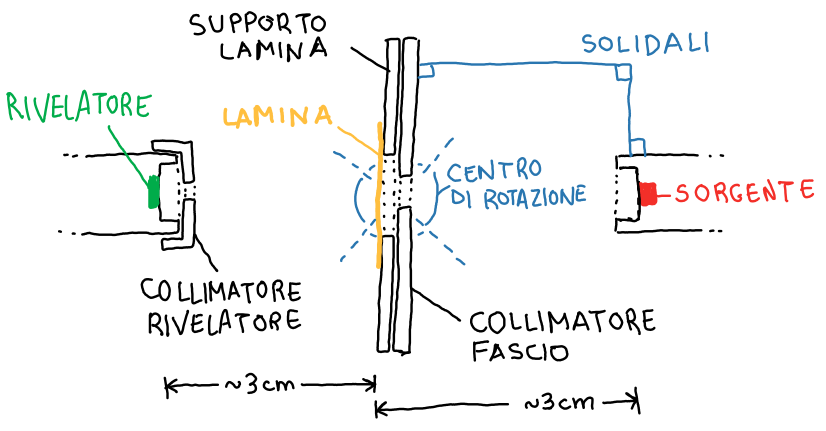
\includegraphics[width=28em]{immagini/schemacamera}
	\caption{\label{fig:schemacamera}
	Schema essenziale dell'apparato di misura.}
\end{figure}

La parte principale del nostro apparato è costituita da una camera a vuoto cilindrica con un diametro interno di  \SI{16.3(1)}{cm} e altezza \SI{8.4(1)}{cm} a cui è collegata la relativa pompa e i vacuometri.
\marginpar{ha senso scrivere l'errore su ste misure ? (Bob)}

Nel centro è possibile inserire un bersaglio che può essere ruotato solidalmente alla sorgente radioattiva $\alpha$
per variare l'angolo tra il proiettile e il rivelatore fisso, un fotodiodo al silicio (vedi \autoref{fig:schemacamera}).
La scheda dell'esperienza afferma che il rivelatore assorbe completamente le particelle $\alpha$,
permettendo di misurarne l'energia.

I bersagli a nostra disposizione sono lamine metalliche di diversi spessori:
\begin{itemize}
	\item oro: \SI{3}{\micro m}, \SI{5}{\micro m}, \SI{20}{\micro m} ($\times$2);
	\item alluminio: \SI{8}{\micro m} ($\times$2);
	\item acciaio: \SI{10}{\micro m};
	\item oro ``calibrato'': \SI2{\micro m};
	\item alluminio ``calibrato'': \SI8{\micro m}.
\end{itemize}
Le lamine ``calibrate'' sono quelle per le quali ci è garantito il valore dello spessore,
le altre lamine erano intese di prova.
Poiché abbiamo saputo solo alla fine dell'esperimento dell'esistenza di questa distinzione,
tutte le misure sono fatte con le lamine ``non calibrate'',
con le lamine ``calibrate'' abbiamo solo fatto delle misure di controllo.

I nostri proiettili sono le particelle $\alpha$ emesse da una sorgente di \am{} con attività \SI{330}{kBq} nel 1990 che si riduce a \SI{315}{kBq} nel 2018.
Possiamo scegliere di collimare il fascio incidente con due collimatori in plastica aventi una fessura rettangolare larga \SI{1}{mm} o \SI{5}{mm} ed altezza di \SI{5}{cm}.
La lamina bersaglio è in ogni caso accoppiata a una maschera circolare di diametro \SI{12}{mm}.
Il fotodiodo ha davanti a sé un collimatore rettangolare di dimensioni $2\times 6$\! mm rotabile a piacere.
\marginpar{spiegare in seguito che lo lasceremo sempre in verticale}

\paragraph{Elettronica di misura}

L'energia dei segnali del fotodiodo è misurata con un circuito preamplificatore-amplificatore-ADC.
Il circuito è triggerato da un discriminatore a soglia in tensione sul segnale del fotodiodo.
L'ADC è a 12 bit e fornisce anche il timestamp dell'evento con un round-time di 1.8 ore.
I segnali triggerati vengono anche contati da un modulo contatore.
Usiamo un timer in modalità bistabile per avviare e fermare contemporaneamente
il contatore e il circuito di misura dell'energia; il tempo è misurato dal conteggio \texttt{clock} del contatore. 


\section{Teoria}

\section{Misura e analisi}

\subsection{Strategia di acquisizione}

\paragraph{Angoli}
\label{spiegazione}
Ci accorgiamo che non siamo in grado di sistemare il coperchio della camera a vuoto esattamente nello stesso punto ogni volta che chiudiamo la camera. Eliminiamo questa sistematica sfruttando il fatto che il coperchio ha un foro che deve essere posizionato al di sopra di un perno. Dopo averlo incastrato lo spingiamo a sinistra e, una volta fatto il vuoto, la pressione atmosferica renderà impossibile spostarlo.
Questo accorgimento ci permette di riposizionare la sorgente nello stesso punto della scala graduata. Cercheremo gli angoli ``veri'' attraverso l'analisi delle nostre misure.
\marginpar{non so come spiegare questa cosa dell'angolo vero con parole migliori}
Riduciamo la parallasse nell'allineamento attaccando un pezzo di carta con una tacca al supporto della sorgente.
\marginpar{spiegare meglio il pezzo di carta (io metterei la foto senza aggiungere altro)}

\paragraph{Energia}
Per acquisire al meglio i segnali amplificati dobbiamo costruire un circuito che sincronizzi il contatore e l'ADC all'inizio e alla fine di ogni acquisizione.
Vogliamo comandare l'inizio e la fine di ogni acquisizione agendo sulla levetta di un timer.
I conteggi vengono effettuati collegando l'uscita TTL del discriminatore ad un generatore di impulsi non retriggerabile, la cui uscita va ad un contatore. Per far partire e fermare un'acquisizione elettronicamente è sufficiente collegare l'uscita del timer allo \emph{start} del contatore e l'\emph{end marker} allo \emph{stop}.
Per fare la stessa cosa con l'ADC colleghiamo l'uscita del timer (con durata impostata su $\infty$) ad un modulo di coincidenze a cui è connessa, ad un altro ingresso, l'uscita TTL del generatore di impulsi convertita in NIM. Il segnale di coincidenza (convertito in TTL) sarà il trigger dell'ADC, che deve arrivare all'omonimo ingresso \SI{1}{\micro s} prima del segnale affinché ne selezioni il picco.
Concludiamo la procedura inserendo i ritardi opportuni.

\paragraph{Precauzioni}
Evitiamo che segnali superiori a \SI{3.3}{V} danneggino l'ADC ponendo un attenuatore da \SI{0.9}{dB} all'uscita dell'amplificatore. Per il trigger non è necessario prendere precauzioni in quanto il convertitore NIM-TTL fornisce un segnale della tensione giusta. \marginpar{misurare?}

\paragraph{Salvataggio dati}
Il circuito descritto nel paragrafo \textbf{Energia} ha una particolarità: quando il crate si accende, il timer si riattiva e riavvia la catena di acquisizione.
Questo accorgimento è particolarmente utile se la corrente dovesse mancare mentre non siamo presenti. In tal caso l'ADC, al ritorno della corrente, registrerebbe i dati nella memoria interna (essendo il computer spento) ed essi sono facilmente recuperabili dopo la riaccensione del computer.


\subsubsection{Taratura ADC}
L'ADC è stata tarata ponendo la sorgente a \SI{0}{\degree} e variando il ritardo sul trigger fino a massimizzare la lettura del segnale. Il risultato di tale misura è presente in \autoref{tara}. Abbiamo acquisito lo spettro a vari angoli e verificato che l'energia delle particelle $\alpha$ non dipendesse dall'angolo in assenza di bersaglio. 
\marginpar{il fit e la figura sono degli scalda posto per sapere come verrà in seguito}
Abbiamo fittato lo spettro a \SI{0}{\degree} con una Gaussiana lasciandone libera anche la normalizzazione.\\
Abbiamo ottenuto:
\begin{align*}
\mu &=3115\pm2 \\
\sigma &= 87\pm2 \\
N &=(1.18\pm0.02)\cdot10^5 \\
\chi^2 &=2313\pm15 \\
\text{dof} &=15 \\
\end{align*}
Il valore elevato del $\chi^2$ mostra chiaramente la non gaussianità del picco osservato.

\begin{figure}[h]
\centering
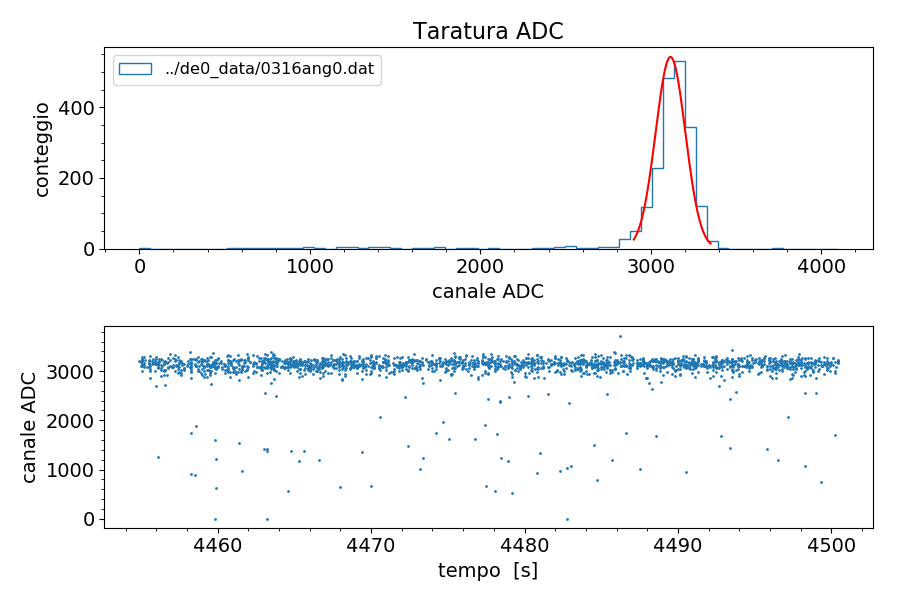
\includegraphics[width=23 em]{immagini/cal_provv}
\caption{Risoluzione in energia dell'ADC. Il pannello superiore mostra l'istogramma dei dati acquisiti con la funzione di fit, quello inferiore mostra il loro valore in funzione del tempo.}
\label{tara}
\end{figure}

\subsection{Pressione}

Variamo la pressione nella camera tenendo la sorgente a \SI{0}{\degree} per cercare in quali condizioni l'aria residua non influisce sulla misura.
Registriamo per ogni valore della pressione il rate di eventi ed il relativo spettro. In \autoref{tab:press} sono presenti i dati ed in \autoref{fig:press} il loro andamento.

\marginpar{qui mi riferisco agli angoli segnati sulla scala graduata, ricordiamoci che gli angoli rispetto al fotodiodo sono altri}

% tabella: angolo || rate || moda spettro (90)%CR -> spiegare quest'ultimo in caption
\marginpar{aggiungere la tabella}

\begin{figure}[h]
\centering
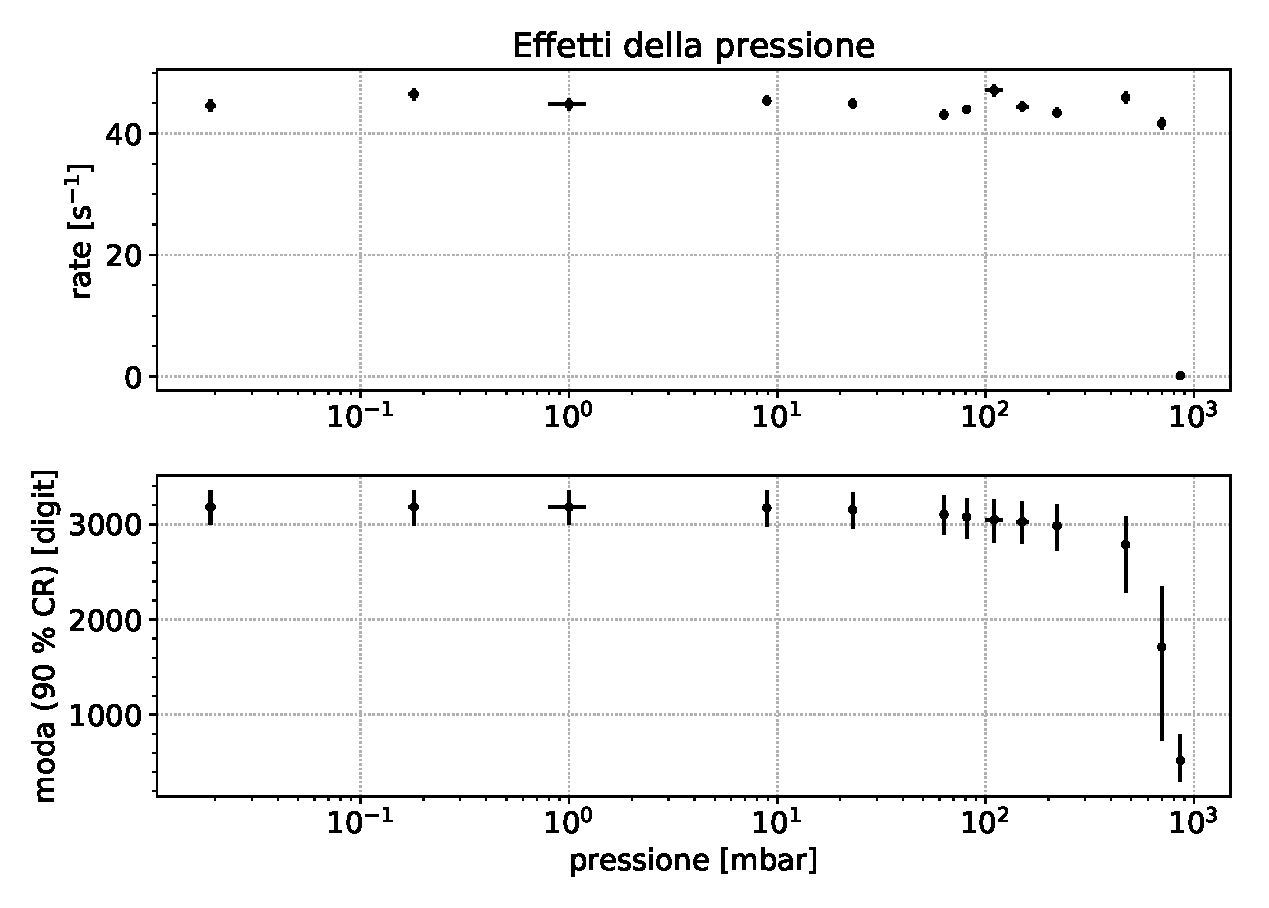
\includegraphics[width=30 em]{immagini/press}
\caption{Effetti della pressione su conteggi e spettri. Il pannello superiore mostra il variare del rate al variare la pressione, quello sottostante contiene la moda dei relativi spettri con errore un intervallo del 90\% di credibilità.}
\label{fig:press}
\end{figure}

\marginpar{Il 90\% di credibilità mi sembra eccessivo come errore. Si vedono i punti che scendono, ma gli errori enormi fanno credere che sia tutto compatibile. 
Ho guardato gli spettri e mi sono accorto che, alzando la pressione, le distro si allargano. Me ne farò una ragione.}

Dal grafico di \autoref{fig:press} non si nota nessuna variazione dei conteggi fino ad \SI{1}{atm}, ma la moda dello spettro inizia a decrescere quando la pressione è maggiore di \SI{200}{mbar}. 
Come atteso, la distribuzione di energia persa dalle particelle $\alpha$ in aria diventa sempre più larga all'aumentare della pressione.
Questo risultato ci assicura una grande indipendenza dalla condizione di vuoto della camera. 
\marginpar{aggiungere questione misure notturne}

\marginpar{secondo me dobbiamo mostrare questa cosa con l'istogramma di alcuni spettri perché dà un'idea più immediata rispetto al fornire l'intervallo di credibilità}

\subsection{Discriminatore}

\begin{figure}
	\hspace{-0.15\textwidth}
	{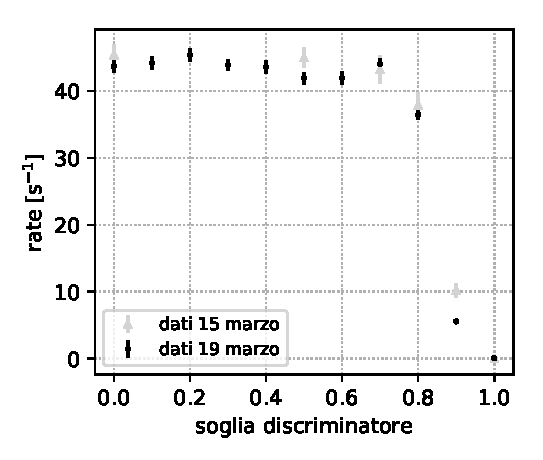
\includegraphics[width=0.6\textwidth]{immagini/soglia}}~
	{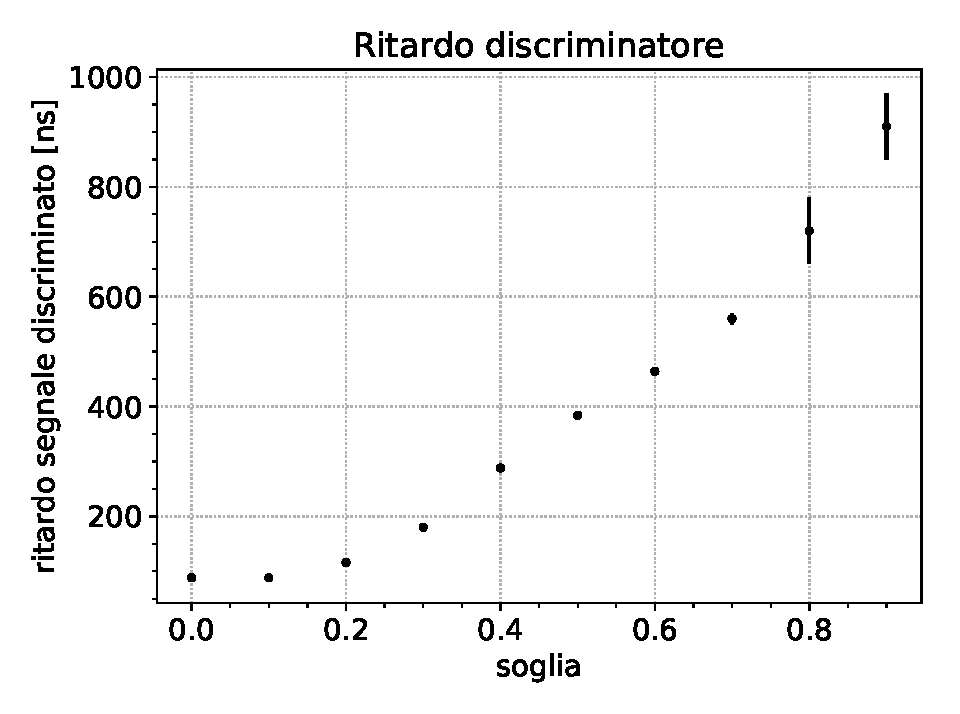
\includegraphics[width=0.6\textwidth]{immagini/ritardo}}
	\caption{\label{fig:sogliaritardo}
	Rate senza bersaglio al variare della soglia del discriminatore (sinistra)
	e ritardo temporale del segnale discriminato rispetto all'ingresso (destra).}
\end{figure}

La manopola di regolazione della soglia del discriminatore non indica l'unità di misura,
però con l'oscilloscopio vediamo che corrisponde circa ai volt quindi supponiamo siano proprio volt.

A \SI0{\degree} senza bersaglio misuriamo il rate al variare della soglia.
Poiché la soglia è in tensione e il segnale del fotodiodo è una curva a campana,
al variare dell'ampiezza del segnale o della soglia
cambia il ritardo del segnale discriminato rispetto a quello in ingresso,
quindi misuriamo anche il ritardo.
Le misure sono riportate in \autoref{fig:sogliaritardo}.
Dal fatto che il ritardo non cambi sulle due soglie più basse
stimiamo che la soglia minima effettiva sia circa \SI{100}{mV}.
Il ritardo introduce un bias verso il basso nelle misure di spettro,
ma non significativo rispetto alla larghezza degli spettri e ad altri problemi esposti di seguito.

% Variamo la soglia del discriminatore collegato al fotodiodo e registriamo il corrispondente rate di eventi a \SI0{\degree} senza collimatori.
% I valori di soglia riportati non hanno unità di misura perché sullo strumento sono solo presenti dei pallini e dei numeri interi.
% Non avendo trovato il manuale dello strumento, ci limitiamo a indicare la posizione del potenziometro.
% Scopriamo (\autoref{fig:soglia}) che il valore della soglia è ininfluente fino a 0.7 e si ha una repentina variazione dopo questo valore.
%
% Per sapere se la soglia ha un effetto minore di quanto misurato dobbiamo aumentare la statistica. I rates misurati hanno (nel migliore dei casi) una precisione del 2\%.
% Siccome il rate diminuisce di molto all'aumentare dell'angolo, le misure ad angoli maggiori avranno un'accuratezza minore. Quindi possiamo affermare che la soglia non avrà alcun effetto sulle misure di rate.
% Pertanto la teniamo a 0 per tutta l'esperienza.


\subsection{Forma del fascio}

Abbiamo fatto delle misure di conteggio a vari angoli con e senza collimatori per studiare la forma del fascio.

\subsubsection{Assenza di collimatori}

La misura in assenza di collimatori ci permette di indagare la forma del fascio di particelle $\alpha$ in uscita dalla sorgente di \am{}.
\marginpar{disegno provvisorio}
Bisogna notare che l'angolo segnato sulla scala graduata non coincide con quello tra la sorgente ed il rivelatore perché il fotodiodo non è al centro della camera a vuoto, inoltre all'aumentare (in modulo) dell'angolo la distanza tra sorgente e rivelatore diminuisce. 
Lo schema di \autoref{fma} illustra la situazione.

\begin{figure}[h]
\centering
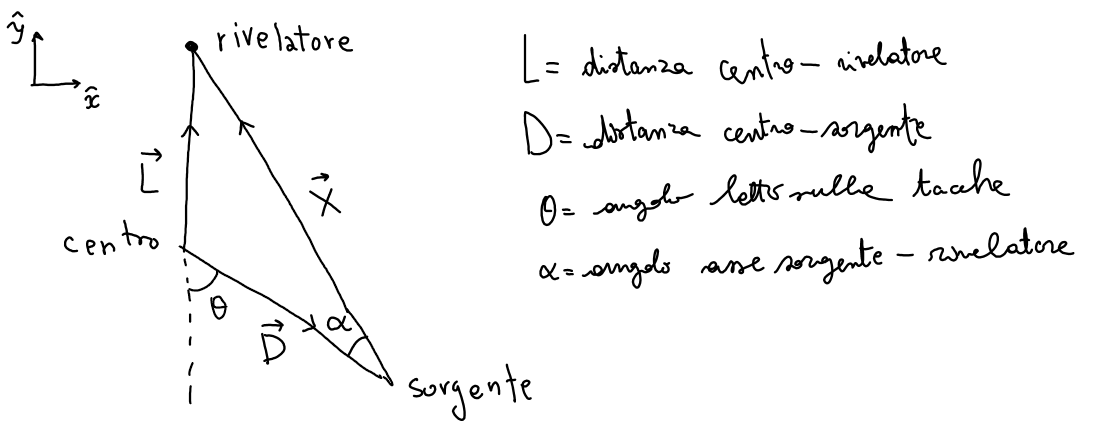
\includegraphics[width=30 em]{immagini/fma_provv}
\caption{Schema raffigurante gli angoli tra rivelatore, centro della camera a vuoto e sorgente.}
\label{fma}
\end{figure}

Applicate le dovute correzioni e usando le variabili di \autoref{fma} troviamo che l'angolo tra rivelatore e sorgente è
\begin{equation}
\cos{\alpha}= -\frac{\vec{X} \cdot \vec{D} }{ |\vec{X}| |\vec{D}| } = \frac{ L \cos{\theta} + D }{ \sqrt{ L^2+2LD\cos{\theta}+D^2  } }.
\end{equation}

Teniamo conto della variazione della distanza al variare dell'angolo moltiplicando ogni rate per $|\vec{X}|^2$.
Tale fattore è giustificato dal fatto che supponiamo isotropa l'emissione di particelle $\alpha$ da parte della sorgente.
Se $C$ è una costante, abbiamo che $$ \frac{dN}{d^3r}=C \implies \frac{dN}{dr}=C 4\pi r^2. $$

\marginpar{A dire il vero non lo so perché. Mi sembra che bisogna dividere per X$^2$ (analogia col campo elettrico). Invece moltiplichiamo. Il grafico ha senso ma non mi torna perché dovrei avere meno eventi all'allontanarmi dal rivelatore ad angolo fissato.}

Il risultato di questa misura è presente in \autoref{fig:form}, invece la \autoref{tab:form} contiene i dati di tale grafico.
Si evince che il fascio ha un'estensione angolare di quasi \SI{50}{\degree}.

\marginpar{inserire tante belle cose}

Useremo queste informazioni (se sarà necessario) nell'analizzare i dati sulla sezione d'urto.

\subsubsection{Collimatore da 5\! mm}

\subsubsection{Collimatore da 1\! mm}

\subsubsection{Collimatore a croce}

\subsection{Fit}

Misuriamo il rate di eventi al variare dell'angolo con i seguenti materiali:
\begin{itemize}
\item oro \SI{3}{\micro m}
\item oro \SI5{\micro m}
\item alluminio \SI8{\micro m}.
\end{itemize}




\subsubsection{Z dell'alluminio}

Comparando i parametri di ampiezza dei fit con l'oro con quello eseguito sull'alluminio, possiamo estrarre lo Z di quest'ultimo. Le ampiezze di fit hanno la forma $$ B=\mathcal{L} \left( \frac {zZ\alpha\hbar c} {2T} \right)^2 = \mathcal{L} A . $$
La nostra luminosità vale $\mathcal{L}=r n_2 l$, in cui $r$ è il rate di particelle incidenti, $n$  è la densità di bersagli e $l$ è lo spessore della targhetta.
Nel nostro caso $n_1$ è uguale per tutte le misure con lo stesso collimatore.   \marginpar{c'è bisogno di precisare perché?}
Da queste considerazioni possiamo trarre lo Z dell'alluminio dalla relazione \eqref{zeta} usando i parametri di fit per i dati con lo stesso collimatore.

\begin{equation}
Z_{\text{al}}=Z_{\text{au}} \sqrt{ \frac{B_{\text{al}}}{B_{\text{au}}} \frac{n_{\text{au}} l_{\text{au}}}{n_{\text{al}} l_{\text{al}}} }
\label{zeta}
\end{equation}

Otteniamo i seguenti risultati:

\begin{align*}
\text{Oro } \SI3{\micro m}&:\\
\text{collimatore } \SI1{mm}&: Z_{\text{al}}=\num{10.4(4)} \\
\text{collimatore } \SI5{mm}&: Z_{\text{al}}=\num{9.2(4)}. \\
\text{Oro } \SI5{\micro m}&:\\
\text{collimatore } \SI1{mm}&: Z_{\text{al}}=\num{13.5(6)} \\
\text{collimatore } \SI5{mm}&: Z_{\text{al}}=\num{70(2)}. \\
\end{align*}

Soltanto una misura è compatibile con lo $Z$ dell'alluminio atteso. Gli altri risultati sono influenzati dallo scattering multiplo all'interno dell'oro, fenomeno praticamente assente nell'alluminio.
L'ultimo risultato è molto lontano dal valore atteso perché lo scattering multiplo influisce pesantemente su una lamina d'oro così spessa e il fatto che il collimatore da \SI5{mm} selezioni più angoli rispetto a quello da \SI1{mm} non fa che peggiorare la situazione.

\end{document}